% Options for packages loaded elsewhere
\PassOptionsToPackage{unicode}{hyperref}
\PassOptionsToPackage{hyphens}{url}
%
\documentclass[
]{article}
\usepackage{amsmath,amssymb}
\usepackage{iftex}
\ifPDFTeX
  \usepackage[T1]{fontenc}
  \usepackage[utf8]{inputenc}
  \usepackage{textcomp} % provide euro and other symbols
\else % if luatex or xetex
  \usepackage{unicode-math} % this also loads fontspec
  \defaultfontfeatures{Scale=MatchLowercase}
  \defaultfontfeatures[\rmfamily]{Ligatures=TeX,Scale=1}
\fi
\usepackage{lmodern}
\ifPDFTeX\else
  % xetex/luatex font selection
\fi
% Use upquote if available, for straight quotes in verbatim environments
\IfFileExists{upquote.sty}{\usepackage{upquote}}{}
\IfFileExists{microtype.sty}{% use microtype if available
  \usepackage[]{microtype}
  \UseMicrotypeSet[protrusion]{basicmath} % disable protrusion for tt fonts
}{}
\makeatletter
\@ifundefined{KOMAClassName}{% if non-KOMA class
  \IfFileExists{parskip.sty}{%
    \usepackage{parskip}
  }{% else
    \setlength{\parindent}{0pt}
    \setlength{\parskip}{6pt plus 2pt minus 1pt}}
}{% if KOMA class
  \KOMAoptions{parskip=half}}
\makeatother
\usepackage{xcolor}
\usepackage[margin=1in]{geometry}
\usepackage{color}
\usepackage{fancyvrb}
\newcommand{\VerbBar}{|}
\newcommand{\VERB}{\Verb[commandchars=\\\{\}]}
\DefineVerbatimEnvironment{Highlighting}{Verbatim}{commandchars=\\\{\}}
% Add ',fontsize=\small' for more characters per line
\usepackage{framed}
\definecolor{shadecolor}{RGB}{248,248,248}
\newenvironment{Shaded}{\begin{snugshade}}{\end{snugshade}}
\newcommand{\AlertTok}[1]{\textcolor[rgb]{0.94,0.16,0.16}{#1}}
\newcommand{\AnnotationTok}[1]{\textcolor[rgb]{0.56,0.35,0.01}{\textbf{\textit{#1}}}}
\newcommand{\AttributeTok}[1]{\textcolor[rgb]{0.13,0.29,0.53}{#1}}
\newcommand{\BaseNTok}[1]{\textcolor[rgb]{0.00,0.00,0.81}{#1}}
\newcommand{\BuiltInTok}[1]{#1}
\newcommand{\CharTok}[1]{\textcolor[rgb]{0.31,0.60,0.02}{#1}}
\newcommand{\CommentTok}[1]{\textcolor[rgb]{0.56,0.35,0.01}{\textit{#1}}}
\newcommand{\CommentVarTok}[1]{\textcolor[rgb]{0.56,0.35,0.01}{\textbf{\textit{#1}}}}
\newcommand{\ConstantTok}[1]{\textcolor[rgb]{0.56,0.35,0.01}{#1}}
\newcommand{\ControlFlowTok}[1]{\textcolor[rgb]{0.13,0.29,0.53}{\textbf{#1}}}
\newcommand{\DataTypeTok}[1]{\textcolor[rgb]{0.13,0.29,0.53}{#1}}
\newcommand{\DecValTok}[1]{\textcolor[rgb]{0.00,0.00,0.81}{#1}}
\newcommand{\DocumentationTok}[1]{\textcolor[rgb]{0.56,0.35,0.01}{\textbf{\textit{#1}}}}
\newcommand{\ErrorTok}[1]{\textcolor[rgb]{0.64,0.00,0.00}{\textbf{#1}}}
\newcommand{\ExtensionTok}[1]{#1}
\newcommand{\FloatTok}[1]{\textcolor[rgb]{0.00,0.00,0.81}{#1}}
\newcommand{\FunctionTok}[1]{\textcolor[rgb]{0.13,0.29,0.53}{\textbf{#1}}}
\newcommand{\ImportTok}[1]{#1}
\newcommand{\InformationTok}[1]{\textcolor[rgb]{0.56,0.35,0.01}{\textbf{\textit{#1}}}}
\newcommand{\KeywordTok}[1]{\textcolor[rgb]{0.13,0.29,0.53}{\textbf{#1}}}
\newcommand{\NormalTok}[1]{#1}
\newcommand{\OperatorTok}[1]{\textcolor[rgb]{0.81,0.36,0.00}{\textbf{#1}}}
\newcommand{\OtherTok}[1]{\textcolor[rgb]{0.56,0.35,0.01}{#1}}
\newcommand{\PreprocessorTok}[1]{\textcolor[rgb]{0.56,0.35,0.01}{\textit{#1}}}
\newcommand{\RegionMarkerTok}[1]{#1}
\newcommand{\SpecialCharTok}[1]{\textcolor[rgb]{0.81,0.36,0.00}{\textbf{#1}}}
\newcommand{\SpecialStringTok}[1]{\textcolor[rgb]{0.31,0.60,0.02}{#1}}
\newcommand{\StringTok}[1]{\textcolor[rgb]{0.31,0.60,0.02}{#1}}
\newcommand{\VariableTok}[1]{\textcolor[rgb]{0.00,0.00,0.00}{#1}}
\newcommand{\VerbatimStringTok}[1]{\textcolor[rgb]{0.31,0.60,0.02}{#1}}
\newcommand{\WarningTok}[1]{\textcolor[rgb]{0.56,0.35,0.01}{\textbf{\textit{#1}}}}
\usepackage{graphicx}
\makeatletter
\def\maxwidth{\ifdim\Gin@nat@width>\linewidth\linewidth\else\Gin@nat@width\fi}
\def\maxheight{\ifdim\Gin@nat@height>\textheight\textheight\else\Gin@nat@height\fi}
\makeatother
% Scale images if necessary, so that they will not overflow the page
% margins by default, and it is still possible to overwrite the defaults
% using explicit options in \includegraphics[width, height, ...]{}
\setkeys{Gin}{width=\maxwidth,height=\maxheight,keepaspectratio}
% Set default figure placement to htbp
\makeatletter
\def\fps@figure{htbp}
\makeatother
\setlength{\emergencystretch}{3em} % prevent overfull lines
\providecommand{\tightlist}{%
  \setlength{\itemsep}{0pt}\setlength{\parskip}{0pt}}
\setcounter{secnumdepth}{-\maxdimen} % remove section numbering
\ifLuaTeX
  \usepackage{selnolig}  % disable illegal ligatures
\fi
\IfFileExists{bookmark.sty}{\usepackage{bookmark}}{\usepackage{hyperref}}
\IfFileExists{xurl.sty}{\usepackage{xurl}}{} % add URL line breaks if available
\urlstyle{same}
\hypersetup{
  pdftitle={Homework 1},
  pdfauthor={Harry Wang},
  hidelinks,
  pdfcreator={LaTeX via pandoc}}

\title{Homework 1}
\author{Harry Wang}
\date{2024-01-22}

\begin{document}
\maketitle

\textbf{Problem 1:}

\textbf{Part i}

\begin{Shaded}
\begin{Highlighting}[]
\NormalTok{x }\OtherTok{=} \FunctionTok{c}\NormalTok{(}\FloatTok{2.7}\NormalTok{,}\FloatTok{4.0}\NormalTok{,}\FloatTok{2.3}\NormalTok{,}\FloatTok{5.4}\NormalTok{,}\SpecialCharTok{{-}}\FloatTok{5.3}\NormalTok{,}\FloatTok{1.8}\NormalTok{,}\SpecialCharTok{{-}}\FloatTok{1.3}\NormalTok{,}\SpecialCharTok{{-}}\FloatTok{2.9}\NormalTok{,}\FloatTok{2.1}\NormalTok{,}\FloatTok{3.9}\NormalTok{,}\SpecialCharTok{{-}}\FloatTok{1.8}\NormalTok{,}\FloatTok{0.4}\NormalTok{,}\SpecialCharTok{{-}}\FloatTok{4.2}\NormalTok{,}\FloatTok{0.5}\NormalTok{,}\SpecialCharTok{{-}}\FloatTok{0.1}\NormalTok{,}\FloatTok{1.5}\NormalTok{,}\SpecialCharTok{{-}}\FloatTok{0.7}\NormalTok{)}
\NormalTok{y }\OtherTok{=} \FunctionTok{c}\NormalTok{(}\FloatTok{1.4}\NormalTok{,}\FloatTok{2.5}\NormalTok{,}\FloatTok{2.6}\NormalTok{,}\FloatTok{5.6}\NormalTok{,}\SpecialCharTok{{-}}\FloatTok{2.2}\NormalTok{,}\FloatTok{0.4}\NormalTok{,}\FloatTok{0.1}\NormalTok{,}\SpecialCharTok{{-}}\FloatTok{3.0}\NormalTok{,}\FloatTok{2.2}\NormalTok{,}\FloatTok{0.9}\NormalTok{,}\SpecialCharTok{{-}}\FloatTok{2.4}\NormalTok{,}\FloatTok{1.6}\NormalTok{,}\SpecialCharTok{{-}}\FloatTok{2.5}\NormalTok{,}\FloatTok{0.1}\NormalTok{,}\SpecialCharTok{{-}}\FloatTok{9.9}\NormalTok{,}\FloatTok{1.1}\NormalTok{,}\SpecialCharTok{{-}}\FloatTok{1.7}\NormalTok{)}
\FunctionTok{cbind}\NormalTok{(x,y)}
\end{Highlighting}
\end{Shaded}

\begin{verbatim}
##          x    y
##  [1,]  2.7  1.4
##  [2,]  4.0  2.5
##  [3,]  2.3  2.6
##  [4,]  5.4  5.6
##  [5,] -5.3 -2.2
##  [6,]  1.8  0.4
##  [7,] -1.3  0.1
##  [8,] -2.9 -3.0
##  [9,]  2.1  2.2
## [10,]  3.9  0.9
## [11,] -1.8 -2.4
## [12,]  0.4  1.6
## [13,] -4.2 -2.5
## [14,]  0.5  0.1
## [15,] -0.1 -9.9
## [16,]  1.5  1.1
## [17,] -0.7 -1.7
\end{verbatim}

\begin{Shaded}
\begin{Highlighting}[]
\FunctionTok{summary}\NormalTok{(x)}
\end{Highlighting}
\end{Shaded}

\begin{verbatim}
##    Min. 1st Qu.  Median    Mean 3rd Qu.    Max. 
## -5.3000 -1.3000  0.5000  0.4882  2.3000  5.4000
\end{verbatim}

\begin{Shaded}
\begin{Highlighting}[]
\FunctionTok{var}\NormalTok{(x)}
\end{Highlighting}
\end{Shaded}

\begin{verbatim}
## [1] 8.673603
\end{verbatim}

\begin{Shaded}
\begin{Highlighting}[]
\FunctionTok{boxplot}\NormalTok{(x,}\AttributeTok{horizontal =} \ConstantTok{TRUE}\NormalTok{, }\AttributeTok{main =} \StringTok{"BOX PLOT X"}\NormalTok{)}
\end{Highlighting}
\end{Shaded}

\includegraphics{Homework1_files/figure-latex/unnamed-chunk-1-1.pdf}

\begin{Shaded}
\begin{Highlighting}[]
\FunctionTok{summary}\NormalTok{(y)}
\end{Highlighting}
\end{Shaded}

\begin{verbatim}
##    Min. 1st Qu.  Median    Mean 3rd Qu.    Max. 
## -9.9000 -2.2000  0.4000 -0.1882  1.6000  5.6000
\end{verbatim}

\begin{Shaded}
\begin{Highlighting}[]
\FunctionTok{var}\NormalTok{(y)}
\end{Highlighting}
\end{Shaded}

\begin{verbatim}
## [1] 11.37985
\end{verbatim}

\begin{Shaded}
\begin{Highlighting}[]
\FunctionTok{boxplot}\NormalTok{(y,}\AttributeTok{horizontal =} \ConstantTok{TRUE}\NormalTok{, }\AttributeTok{main =} \StringTok{"BOX PLOT Y"}\NormalTok{)}
\end{Highlighting}
\end{Shaded}

\includegraphics{Homework1_files/figure-latex/unnamed-chunk-1-2.pdf}

For x, the box-plot is skewed left. There are no outliers.\\
For y, the box-plot is skewed right. There is one outlier which is -9.9.

\textbf{Part ii}

\begin{Shaded}
\begin{Highlighting}[]
\FunctionTok{plot}\NormalTok{(x,y)}
\end{Highlighting}
\end{Shaded}

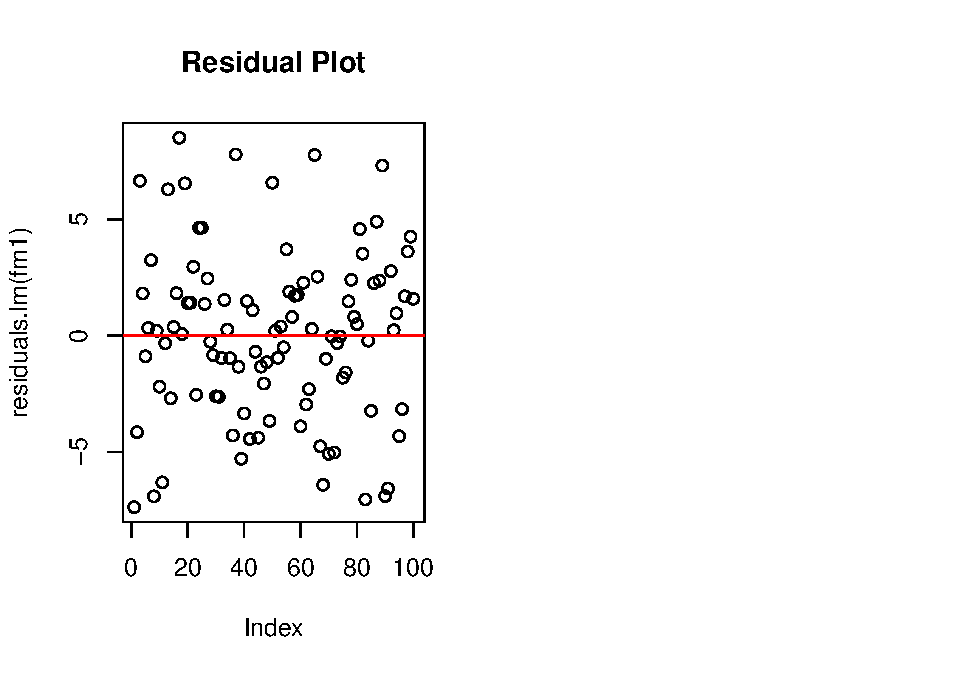
\includegraphics{Homework1_files/figure-latex/unnamed-chunk-2-1.pdf}

\begin{Shaded}
\begin{Highlighting}[]
\FunctionTok{cor}\NormalTok{(x,y)}
\end{Highlighting}
\end{Shaded}

\begin{verbatim}
## [1] 0.6289777
\end{verbatim}

The scatter plot for x and y, the linear association between x and y is

\textbf{Part iii}

Since a paired observation is usually considered to be an outlier if one
if its two coordinators is an outlier. Since there is one in y, the
outlier is (-0.1,-9.9). This is the correlation coefficient after
removing the outlier.

\begin{Shaded}
\begin{Highlighting}[]
\NormalTok{x }\OtherTok{=} \FunctionTok{c}\NormalTok{(}\FloatTok{2.7}\NormalTok{,}\FloatTok{4.0}\NormalTok{,}\FloatTok{2.3}\NormalTok{,}\FloatTok{5.4}\NormalTok{,}\SpecialCharTok{{-}}\FloatTok{5.3}\NormalTok{,}\FloatTok{1.8}\NormalTok{,}\SpecialCharTok{{-}}\FloatTok{1.3}\NormalTok{,}\SpecialCharTok{{-}}\FloatTok{2.9}\NormalTok{,}\FloatTok{2.1}\NormalTok{,}\FloatTok{3.9}\NormalTok{,}\SpecialCharTok{{-}}\FloatTok{1.8}\NormalTok{,}\FloatTok{0.4}\NormalTok{,}\SpecialCharTok{{-}}\FloatTok{4.2}\NormalTok{,}\FloatTok{0.5}\NormalTok{,}\FloatTok{1.5}\NormalTok{,}\SpecialCharTok{{-}}\FloatTok{0.7}\NormalTok{)}
\NormalTok{y }\OtherTok{=} \FunctionTok{c}\NormalTok{(}\FloatTok{1.4}\NormalTok{,}\FloatTok{2.5}\NormalTok{,}\FloatTok{2.6}\NormalTok{,}\FloatTok{5.6}\NormalTok{,}\SpecialCharTok{{-}}\FloatTok{2.2}\NormalTok{,}\FloatTok{0.4}\NormalTok{,}\FloatTok{0.1}\NormalTok{,}\SpecialCharTok{{-}}\FloatTok{3.0}\NormalTok{,}\FloatTok{2.2}\NormalTok{,}\FloatTok{0.9}\NormalTok{,}\SpecialCharTok{{-}}\FloatTok{2.4}\NormalTok{,}\FloatTok{1.6}\NormalTok{,}\SpecialCharTok{{-}}\FloatTok{2.5}\NormalTok{,}\FloatTok{0.1}\NormalTok{,}\FloatTok{1.1}\NormalTok{,}\SpecialCharTok{{-}}\FloatTok{1.7}\NormalTok{)}
\FunctionTok{cor}\NormalTok{(x,y)}
\end{Highlighting}
\end{Shaded}

\begin{verbatim}
## [1] 0.8822511
\end{verbatim}

\textbf{Part iv}

\begin{Shaded}
\begin{Highlighting}[]
\FunctionTok{plot}\NormalTok{(x,y, }\AttributeTok{main =} \StringTok{"After"}\NormalTok{)}
\end{Highlighting}
\end{Shaded}

\includegraphics{Homework1_files/figure-latex/unnamed-chunk-4-1.pdf}

\begin{Shaded}
\begin{Highlighting}[]
\NormalTok{x }\OtherTok{=} \FunctionTok{c}\NormalTok{(}\FloatTok{2.7}\NormalTok{,}\FloatTok{4.0}\NormalTok{,}\FloatTok{2.3}\NormalTok{,}\FloatTok{5.4}\NormalTok{,}\SpecialCharTok{{-}}\FloatTok{5.3}\NormalTok{,}\FloatTok{1.8}\NormalTok{,}\SpecialCharTok{{-}}\FloatTok{1.3}\NormalTok{,}\SpecialCharTok{{-}}\FloatTok{2.9}\NormalTok{,}\FloatTok{2.1}\NormalTok{,}\FloatTok{3.9}\NormalTok{,}\SpecialCharTok{{-}}\FloatTok{1.8}\NormalTok{,}\FloatTok{0.4}\NormalTok{,}\SpecialCharTok{{-}}\FloatTok{4.2}\NormalTok{,}\FloatTok{0.5}\NormalTok{,}\SpecialCharTok{{-}}\FloatTok{0.1}\NormalTok{,}\FloatTok{1.5}\NormalTok{,}\SpecialCharTok{{-}}\FloatTok{0.7}\NormalTok{)}
\NormalTok{y }\OtherTok{=} \FunctionTok{c}\NormalTok{(}\FloatTok{1.4}\NormalTok{,}\FloatTok{2.5}\NormalTok{,}\FloatTok{2.6}\NormalTok{,}\FloatTok{5.6}\NormalTok{,}\SpecialCharTok{{-}}\FloatTok{2.2}\NormalTok{,}\FloatTok{0.4}\NormalTok{,}\FloatTok{0.1}\NormalTok{,}\SpecialCharTok{{-}}\FloatTok{3.0}\NormalTok{,}\FloatTok{2.2}\NormalTok{,}\FloatTok{0.9}\NormalTok{,}\SpecialCharTok{{-}}\FloatTok{2.4}\NormalTok{,}\FloatTok{1.6}\NormalTok{,}\SpecialCharTok{{-}}\FloatTok{2.5}\NormalTok{,}\FloatTok{0.1}\NormalTok{,}\SpecialCharTok{{-}}\FloatTok{9.9}\NormalTok{,}\FloatTok{1.1}\NormalTok{,}\SpecialCharTok{{-}}\FloatTok{1.7}\NormalTok{)}
\FunctionTok{plot}\NormalTok{(x,y, }\AttributeTok{main =} \StringTok{"Before"}\NormalTok{)}
\end{Highlighting}
\end{Shaded}

\includegraphics{Homework1_files/figure-latex/unnamed-chunk-4-2.pdf}

You can visually see the ``Before'' graph has an outlier on the bottom
which causes a huge decrease on the correlation coefficient. But the
``After'', you can not visually see any outliers.

\textbf{Part v} The correlation coefficient after the removal of the
outlier went from 0.6289777 to 0.8822511. The correlation coefficient
measures the degree of linear association between vectors x and y. So
removing of the outlier increased the linear association between vectors
x and y.

\textbf{Part vi}

\begin{Shaded}
\begin{Highlighting}[]
\FunctionTok{qqnorm}\NormalTok{(x, }\AttributeTok{main =} \StringTok{"Normal QQ plots (x)"}\NormalTok{)}
\FunctionTok{qqline}\NormalTok{(x)}
\end{Highlighting}
\end{Shaded}

\includegraphics{Homework1_files/figure-latex/unnamed-chunk-5-1.pdf}

\begin{Shaded}
\begin{Highlighting}[]
\FunctionTok{qqnorm}\NormalTok{(y, }\AttributeTok{main =} \StringTok{"Normal QQ plots (y)"}\NormalTok{)}
\FunctionTok{qqline}\NormalTok{(y)}
\end{Highlighting}
\end{Shaded}

\includegraphics{Homework1_files/figure-latex/unnamed-chunk-5-2.pdf}

The one that is more likely to be of normal distribution is x because it
is more linear. Normally distributed data appears as roughly a straight
line.

\begin{Shaded}
\begin{Highlighting}[]
\NormalTok{x }\OtherTok{=} \FunctionTok{c}\NormalTok{(}\FloatTok{2.7}\NormalTok{,}\FloatTok{4.0}\NormalTok{,}\FloatTok{2.3}\NormalTok{,}\FloatTok{5.4}\NormalTok{,}\SpecialCharTok{{-}}\FloatTok{5.3}\NormalTok{,}\FloatTok{1.8}\NormalTok{,}\SpecialCharTok{{-}}\FloatTok{1.3}\NormalTok{,}\SpecialCharTok{{-}}\FloatTok{2.9}\NormalTok{,}\FloatTok{2.1}\NormalTok{,}\FloatTok{3.9}\NormalTok{,}\SpecialCharTok{{-}}\FloatTok{1.8}\NormalTok{,}\FloatTok{0.4}\NormalTok{,}\SpecialCharTok{{-}}\FloatTok{4.2}\NormalTok{,}\FloatTok{0.5}\NormalTok{,}\FloatTok{1.5}\NormalTok{,}\SpecialCharTok{{-}}\FloatTok{0.7}\NormalTok{,}\SpecialCharTok{{-}}\FloatTok{0.1}\NormalTok{)}
\NormalTok{y }\OtherTok{=} \FunctionTok{c}\NormalTok{(}\FloatTok{1.4}\NormalTok{,}\FloatTok{2.5}\NormalTok{,}\FloatTok{2.6}\NormalTok{,}\FloatTok{5.6}\NormalTok{,}\SpecialCharTok{{-}}\FloatTok{2.2}\NormalTok{,}\FloatTok{0.4}\NormalTok{,}\FloatTok{0.1}\NormalTok{,}\SpecialCharTok{{-}}\FloatTok{3.0}\NormalTok{,}\FloatTok{2.2}\NormalTok{,}\FloatTok{0.9}\NormalTok{,}\SpecialCharTok{{-}}\FloatTok{2.4}\NormalTok{,}\FloatTok{1.6}\NormalTok{,}\SpecialCharTok{{-}}\FloatTok{2.5}\NormalTok{,}\FloatTok{0.1}\NormalTok{,}\FloatTok{1.1}\NormalTok{,}\SpecialCharTok{{-}}\FloatTok{1.7}\NormalTok{)}
\FunctionTok{qqnorm}\NormalTok{(x, }\AttributeTok{main =} \StringTok{"Normal QQ plots (x) No Outliers"}\NormalTok{)}
\FunctionTok{qqline}\NormalTok{(x)}
\end{Highlighting}
\end{Shaded}

\includegraphics{Homework1_files/figure-latex/unnamed-chunk-6-1.pdf}

\begin{Shaded}
\begin{Highlighting}[]
\FunctionTok{qqnorm}\NormalTok{(y, }\AttributeTok{main =} \StringTok{"Normal QQ plots (y) No Outliers"}\NormalTok{)}
\FunctionTok{qqline}\NormalTok{(y)}
\end{Highlighting}
\end{Shaded}

\includegraphics{Homework1_files/figure-latex/unnamed-chunk-6-2.pdf}

After removing outliers, it seems like x still the one that is more
likely to be normal distributed.

\textbf{Problem 2}

P(\textbar Z\textbar\textgreater1) = 0.3173105\\
P(\textbar Z\textbar\textgreater2) = 0.04550026\\
P(\textbar Z\textbar\textgreater3) = 0.002699796\\
P(Z ≤ z0.1/2) = 0.05\\
P(Z ≤ z1−0.1/2) = 0.950\\
P(z0.1/2 ≤ Z ≤ z1−0.1/2) = 0.900

\begin{Shaded}
\begin{Highlighting}[]
\FunctionTok{pnorm}\NormalTok{(}\SpecialCharTok{{-}}\DecValTok{1}\NormalTok{) }\SpecialCharTok{*} \DecValTok{2}
\end{Highlighting}
\end{Shaded}

\begin{verbatim}
## [1] 0.3173105
\end{verbatim}

\begin{Shaded}
\begin{Highlighting}[]
\FunctionTok{pnorm}\NormalTok{(}\SpecialCharTok{{-}}\DecValTok{2}\NormalTok{) }\SpecialCharTok{*} \DecValTok{2}
\end{Highlighting}
\end{Shaded}

\begin{verbatim}
## [1] 0.04550026
\end{verbatim}

\begin{Shaded}
\begin{Highlighting}[]
\FunctionTok{pnorm}\NormalTok{(}\SpecialCharTok{{-}}\DecValTok{3}\NormalTok{) }\SpecialCharTok{*} \DecValTok{2}
\end{Highlighting}
\end{Shaded}

\begin{verbatim}
## [1] 0.002699796
\end{verbatim}

\begin{Shaded}
\begin{Highlighting}[]
\FunctionTok{curve}\NormalTok{(dnorm, }\SpecialCharTok{{-}}\FloatTok{3.5}\NormalTok{, }\FloatTok{3.5}\NormalTok{, }\AttributeTok{lwd=}\DecValTok{2}\NormalTok{, }\AttributeTok{axes =} \ConstantTok{FALSE}\NormalTok{, }\AttributeTok{xlab =} \StringTok{""}\NormalTok{, }\AttributeTok{ylab =} \StringTok{""}\NormalTok{)}
\FunctionTok{axis}\NormalTok{(}\DecValTok{1}\NormalTok{, }\AttributeTok{at =} \SpecialCharTok{{-}}\DecValTok{3}\SpecialCharTok{:}\DecValTok{3}\NormalTok{, }\AttributeTok{labels =} \FunctionTok{c}\NormalTok{(}\StringTok{"{-}3"}\NormalTok{, }\StringTok{"{-}2"}\NormalTok{, }\StringTok{"{-}1"}\NormalTok{, }\StringTok{"0"}\NormalTok{, }\StringTok{"1"}\NormalTok{, }\StringTok{"2"}\NormalTok{, }\StringTok{"3"}\NormalTok{))}
\FunctionTok{abline}\NormalTok{(}\AttributeTok{v=} \DecValTok{1}\NormalTok{, }\AttributeTok{col=}\StringTok{"blue"}\NormalTok{)}
\FunctionTok{abline}\NormalTok{(}\AttributeTok{v=} \DecValTok{2}\NormalTok{, }\AttributeTok{col=}\StringTok{"blue"}\NormalTok{)}
\FunctionTok{abline}\NormalTok{(}\AttributeTok{v=} \DecValTok{3}\NormalTok{, }\AttributeTok{col=}\StringTok{"blue"}\NormalTok{)}
\FunctionTok{abline}\NormalTok{(}\AttributeTok{v=} \SpecialCharTok{{-}}\FloatTok{1.645}\NormalTok{, }\AttributeTok{col=}\StringTok{"blue"}\NormalTok{)}
\FunctionTok{abline}\NormalTok{(}\AttributeTok{v=} \FloatTok{1.645}\NormalTok{, }\AttributeTok{col=}\StringTok{"blue"}\NormalTok{)}
\FunctionTok{abline}\NormalTok{(}\AttributeTok{v=} \DecValTok{1}\NormalTok{, }\AttributeTok{col=}\StringTok{"blue"}\NormalTok{)}
\end{Highlighting}
\end{Shaded}

\includegraphics{Homework1_files/figure-latex/unnamed-chunk-7-1.pdf}

\textbf{Problem 3}

P(X ≤ F −1(α/2))

Meaning: This probability represents the likelihood that the random
variable is less than or equal to the value at which the cumulative
distribution function F(X) reaches (α/2). Essentially, it's the
probability of X being in the lower tail of its distribution, up to the
α/2 quantile.

Numerical Value: F(F\^{}(-1)(α/2)) = α/2.

P(X \textgreater{} F −1(1 − α/2))

Meaning: This is the probability that X is greater than the value at
which the CDF F(X) reaches 1- α/2 . It represents the probability of X
being in the upper tail of its distribution, beyond the 1 - α/2
quantile.

Numerical Value: 1 - F(F\^{}(-1)(1 − α/2)) = 1 - (1 - α/2) = α/2.

PF −1(α/2) ≤ X ≤ F −1(1 − α/2) = This probability indicates the
likelihood that X falls between the α/2 and 1 - α/2 quantiles of its
distribution. It essentially measures the probability of X being within
the central 1-α portion of its distribution.

Numerical Value: F(F\^{}(-1)(1 − α/2)) - F(F\^{}(-1)(α/2)) = (1 - α/2) -
(α/2) = 1 - α.

In summary, as α decreases, the probabilities of X being in the extreme
tails of its distribution decrease, while the probability of X falling
within a wider central interval increases.

\textbf{Problem 4}

Centralization:

\(\sum_{i=1}^{n} (x_i - x)\) = \(\sum_{i=1}^{n} ((x_i) - nx)\)\\
\(\sum_{i=1}^{n} (x_i - x)\) = \(\sum_{i=1}^{n} x_i - n\) (1/n
\(\sum_{i=1}^{n} x_i)\) = \(\sum_{i=1}^{n} x_i\) -
\(\sum_{i=1}^{n} x_i\) = 0

Square of the Sum:

\((\sum_{i=1}^{n} x_i)^2\) = \(\sum_{i=1}^{n} x_i\) x
\(\sum_{i=1}^{n} x_i^2\) = \((\sum_{i=1}^{n} x_i)^2\) + 2
\(\sum_{1<=i<=j<=n}^{n} x_i x_j\)

So, the left side is equal to the right side, and the equation is
proven.

Sum of Squares:

(\(\sum_{i=1}^{n} x_i^2\))/n = (n \(\sum_{i=1}^{n} x_i^2\))/n\^{}2 = 1/n
\(\sum_{i=1}^{n} x_i^2\))\\
(\(\sum_{i=1}^{n} x_i\))/n)\^{}2 = (x)\^{}2\\
1/n (\(\sum_{i=1}^{n} x_i^2\)) \textgreater= (x)\^{}2

So, the inequality is proven.

Sum of Squared Distances:

\(\sum_{i=1}^{n} (x_i - x)^2\) = \(\sum_{i=1}^{n} (x_i^2 - 2x_ix +x^2)\)
= \(\sum_{i=1}^{n} x_i^2\) - 2x \(\sum_{i=1}^{n} x_i\) +
\(\sum_{i=1}^{n} (x^2)\) = \(\sum_{i=1}^{n} (x_i^2 - 2nx^2 +nx^2)\) =
\(\sum_{i=1}^{n} (x_i^2 - nx^2)\)

So, the left side is equal to the right side, and the equation is
proven.

\end{document}
